\immediate\write18{tex tqft.dtx}
\documentclass{article}
\usepackage{tikz}
\usetikzlibrary{shapes.geometric}
\usepackage{tqft}

\makeatletter
\pgfdeclareshape{test shape}{
  \savedanchor{\centerpoint}{
    \pgfmoveto{\pgfqpoint{0pt}{0pt}}
    \pgfgetlastxy{\my@x}{\my@y}
\pgftransformyscale{-1}\pgftransformrotate{90}\pgftransformshift{\pgfqpoint{1cm}{1cm}}
    \pgfmoveto{\pgfqpoint{0pt}{0pt}}
    \pgfgetlastxy{\my@xa}{\my@ya}
    \pgf@x=-\my@x\relax
    \pgf@y=-\my@y\relax
    \advance\pgf@x by \my@xa\relax
    \advance\pgf@y by \my@ya\relax
%    \showthe\pgf@x
%    \showthe\pgf@y
  }
  \anchor{center}{\centerpoint}
\backgroundpath{
\pgftransformyscale{-1}\pgftransformrotate{90}
  \pgf@process{\pgfqpoint{0pt}{0pt}}
  \pgfpathmoveto{\pgfqpoint{0pt}{0pt}}
  \pgfpathlineto{\pgfqpoint{1cm}{0pt}}
    \pgfpathellipse{\pgfqpoint{0pt}{0pt}}{\pgfqpoint{1cm}{0pt}}{\pgfqpoint{0pt}{2cm}}
  }
}
\makeatother

\begin{document}
\begin{tikzpicture}
\node[tqft pair of pants,draw,circle width=2cm,circle depth=1cm,cobordism height=8cm,boundary separation=2cm] {};
\end{tikzpicture}
\end{document}

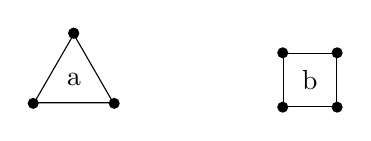
\begin{tikzpicture}
\node[regular polygon,regular polygon sides=3,draw] (a) {a};
\node[regular polygon,regular polygon sides=4,draw] (b) at (3,0) {b};
\foreach \k in {1,...,4} {
  \fill (a.corner \k) circle[radius=2pt];
}
\foreach \k in {1,...,4} {
  \fill (b.corner \k) circle[radius=2pt];
}
\end{tikzpicture}

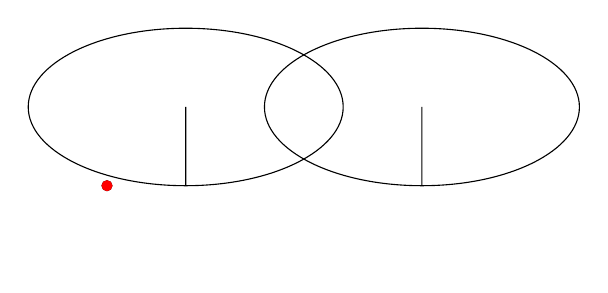
\begin{tikzpicture}
\fill (0,0) circle[radius=2pt];
\node[test shape,draw] (a) {};
\node[test shape,draw] (b) at (3,0) {};
\fill[red] (a) circle[radius=2pt];
\end{tikzpicture}

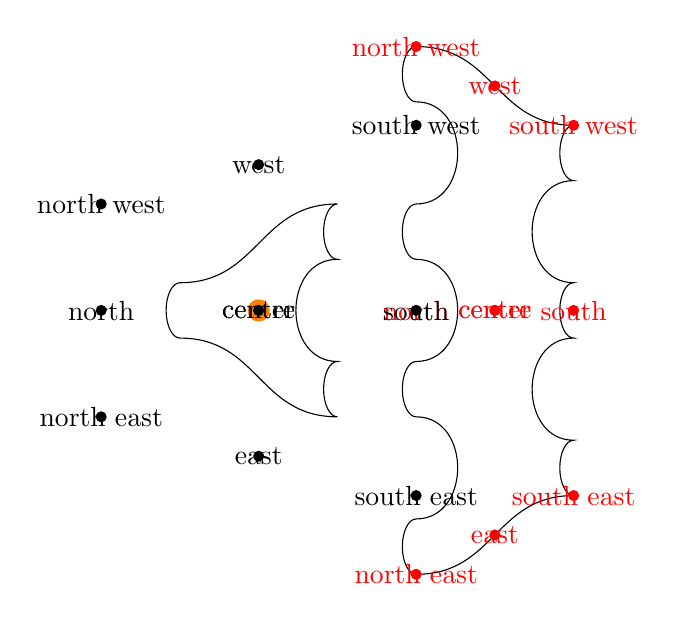
\begin{tikzpicture}[tqft/flow={east}]
\fill[orange] (0,0) circle[radius=4pt];
\node[tqft,pair of pants,draw,outer sep=1cm] (a) at (0,0) {};
\node[tqft,incoming boundary components=4,outgoing boundary components=3,offset=.5,draw] (b) at (3,0) {};
%\node[tqft,pair of pants,draw,red] (b) at (1,0) {};
%\node[tqft,pair of pants,draw,green] (c) at (0,1) {};
%\node[tqft,pair of pants,draw,blue] (d) at (-1,0) {};
%\fill (a.incoming boundary 1) circle[radius=2pt];
%\fill[red] (b.incoming boundary 1) circle[radius=2pt];
%\fill[green] (c.incoming boundary 1) circle[radius=2pt];
%\fill[blue] (d.incoming boundary 1) circle[radius=2pt];
\foreach \anchor in {
  centre,
  center,
  north,
  south,
  east,
  north west,
  south west,
  north east,
  south east,
  west%
} {
\foreach \node/\colour in {
    a/black,
    b/red%,
%    c/green,
%    d/blue%
}{
\edef\command{\noexpand\fill[\colour] (\node.\anchor) circle[radius=2pt] node {\anchor};}
\command
}
}
\end{tikzpicture}


\begin{tikzpicture}
\node[draw,outer sep=1cm] (a) {a};
\fill (a.north) circle[radius=2pt];
\end{tikzpicture}

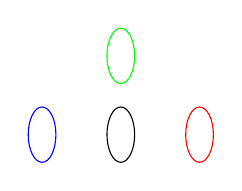
\begin{tikzpicture}[tqft/flow={east}]
\node[tqft,boundary circle,draw] at (0,0) {};
\node[tqft,boundary circle,draw,red] at (1,0) {};
\node[tqft,boundary circle,draw,green] at (0,1) {};
\node[tqft,boundary circle,draw,blue] at (-1,0) {};
\end{tikzpicture}

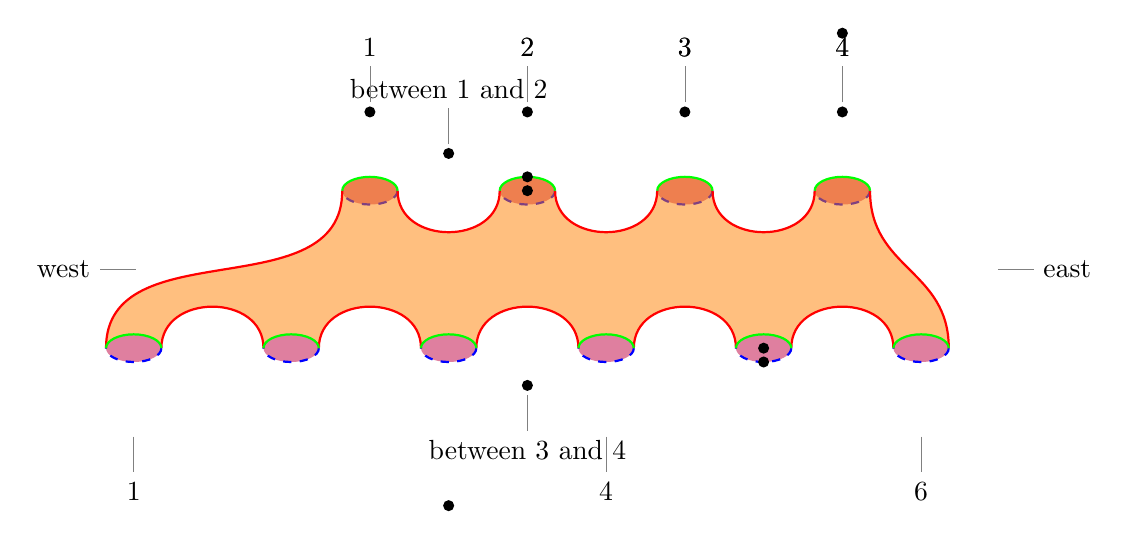
\begin{tikzpicture}[every tqft/.style={cobordism style={draw,thick,red}}]
 \node[
   tqft,
   fill=orange,
   fill opacity=.5,
   boundary style={fill=purple},
   cobordism style={draw,thick,red},
   boundary lower style={draw,dashed,thick,blue},
   boundary upper style={draw,green,thick},
   incoming boundary components=4,
   outgoing boundary components=6,
   offset=-1.5,
   outer sep=1cm,
 ] (a) {};
 \fill (a incoming 2.90) circle[radius=2pt];
 \fill (a outgoing 5.270) circle[radius=2pt];
 \fill (a incoming 2.centre) circle[radius=2pt];
 \fill (a outgoing 5.centre) circle[radius=2pt];
 \fill (a incoming 4.above) circle[radius=2pt];
 \fill (a outgoing 3.below) circle[radius=2pt];
 \fill (a.after incoming boundary 1) circle[radius=2pt] node[pin=north:between 1 and 2] {};
 \fill (a.after outgoing boundary 3) circle[radius=2pt] node[pin=south:between 3 and 4] {};
 \fill (a.incoming boundary 1) circle[radius=2pt] node[pin=north:1] {};
 \fill (a.incoming boundary 2) circle[radius=2pt] node[pin=north:2] {};
 \fill (a.incoming boundary 3) circle[radius=2pt] node[pin=north:3] {};
 \fill (a.incoming boundary 4) circle[radius=2pt] node[pin=north:4] {};
 \node[pin=north:2] at (a.incoming boundary 2) {};
 \node[pin=north:3] at (a.incoming boundary 3) {};
 \node[pin=north:4] at (a.incoming boundary 4) {};
 \node[pin=south:1] at (a.outgoing boundary 1) {};
 \node[pin=south:4] at (a.outgoing boundary 4) {};
 \node[pin=south:6] at (a.outgoing boundary 6) {};
\node[pin=west:west] at (a.west) {};
\node[pin=east:east] at (a.east) {};
 \end{tikzpicture}

\begin{tikzpicture}[every tqft/.style={cobordism style={draw,thick,red}}]
 \node[
   tqft,
   fill=orange,
   fill opacity=.5,
   boundary style={fill=purple},
   cobordism style={draw,thick,red},
   boundary lower style={draw,dashed,thick,blue},
   boundary upper style={draw,green,thick},
   incoming boundary components=0,
   outgoing boundary components=6,
   offset=-1.5,
   outer sep=1cm,
 ] (aa) {hello world};
% \fill (aa incoming 2.90) circle[radius=2pt];
 \fill (aa outgoing 5.270) circle[radius=2pt];
% \fill (aa incoming 2.centre) circle[radius=2pt];
 \fill (aa outgoing 5.centre) circle[radius=2pt];
% \fill (aa incoming 4.above) circle[radius=2pt];
 \fill (aa outgoing 3.below) circle[radius=2pt];
 \fill (aa.incoming boundary 1) circle[radius=2pt] node[pin=north:1] {};
 \fill (aa.incoming boundary 2) circle[radius=2pt] node[pin=north:2] {};
 \fill (aa.incoming boundary 3) circle[radius=2pt] node[pin=north:3] {};
 \fill (aa.incoming boundary 4) circle[radius=2pt] node[pin=north:4] {};
 \node[pin=north:2] at (aa.incoming boundary 2) {};
 \node[pin=north:3] at (aa.incoming boundary 3) {};
 \node[pin=north:4] at (aa.incoming boundary 4) {};
 \node[pin=south:1] at (aa.outgoing boundary 1) {};
 \node[pin=south:4] at (aa.outgoing boundary 4) {};
 \node[pin=south:6] at (aa.outgoing boundary 6) {};
\fill[cyan] (0,0) circle[radius=3pt];
\node[pin=west:west] at (aa.west) {};
\node[pin=east:east] at (aa.east) {};
\node[pin=north:north] at (aa.north) {};
 \end{tikzpicture}

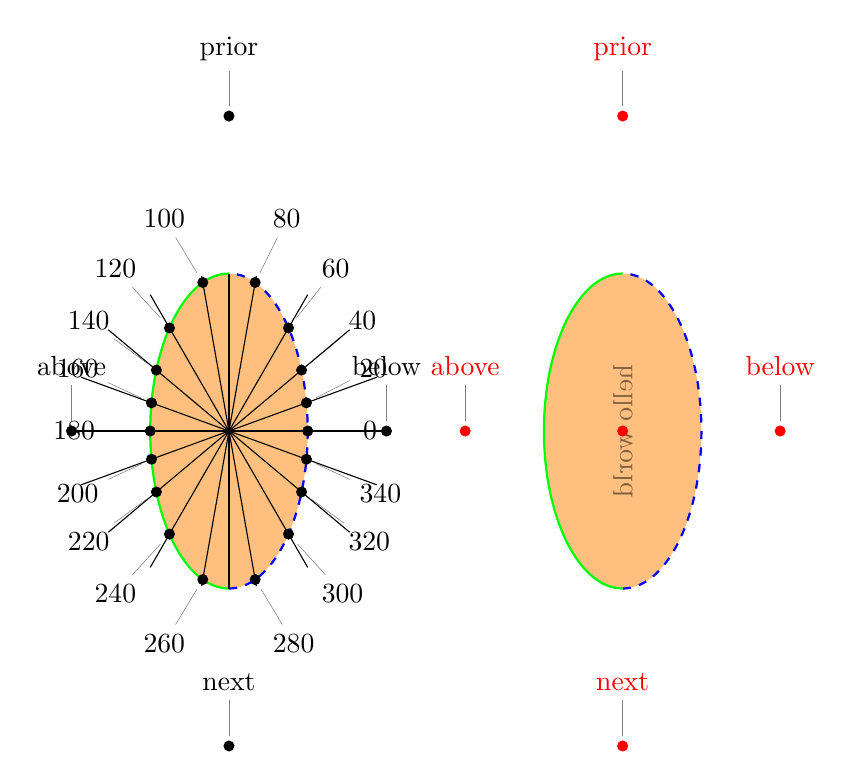
\begin{tikzpicture}[tqft/flow={east},every tqft/.style={cobordism style={draw,thick,red}}]
 \node[
   tqft,
   boundary circle,
   circle width=2cm,
   circle depth=1cm,
   boundary separation=4cm,
   fill=orange,
   fill opacity=.5,
   boundary style={fill=purple},
   cobordism style={draw,thick,red},
   boundary lower style={draw,dashed,thick,blue},
   boundary upper style={draw,green,thick},
   incoming boundary components=4,
   outgoing boundary components=6,
   offset=-1.5,
 ] (a) {};
 \node[
   tqft,
   boundary circle,
   circle width=2cm,
   circle depth=1cm,
   boundary separation=4cm,
   fill=orange,
   fill opacity=.5,
   boundary style={fill=purple},
   cobordism style={draw,thick,red},
   boundary lower style={draw,dashed,thick,blue},
   boundary upper style={draw,green,thick},
   incoming boundary components=4,
   outgoing boundary components=6,
   offset=-1.5,
 ] at (5,0) (b) {hello world};
\fill[red] (b.centre) circle[radius=2pt];
 \fill[red] (b.next) circle[radius=2pt] node[pin=north:next] {};
 \fill[red] (b.prior) circle[radius=2pt] node[pin=north:prior] {};
 \fill[red] (b.above) circle[radius=2pt] node[pin=north:above] {};
 \fill[red] (b.below) circle[radius=2pt] node[pin=north:below] {};
 \fill (a.next) circle[radius=2pt] node[pin=north:next] {};
 \fill (a.prior) circle[radius=2pt] node[pin=north:prior] {};
 \fill (a.above) circle[radius=2pt] node[pin=north:above] {};
 \fill (a.below) circle[radius=2pt] node[pin=north:below] {};
 \draw (0,0) -- (90:2);
 \draw (0,0) -- (0:2);
 \draw (0,0) -- (180:2);
 \draw (0,0) -- (270:2);
\foreach \ang in {0,20,...,340} {
 \fill (a.\ang) circle[radius=2pt] node[pin=\ang:\ang] {};
 \draw (0,0) -- (\ang:2);
}
 \end{tikzpicture}

\end{document}

% Local Variables:
% tex-output-type: "pdf18"
% End: